\subsection{Alumno curso académico}

  \subsubsection{Listar}

  \paragraph{}La aplicación permite generar listados de los alumnos, de un
  determinado curso académico, que pertenezcan al centro que gestiona el usuario
  \textit{Administrador de centro} que ha accedido a la aplicación.

  \paragraph{}Para generar este listado, primero será necesario establecer el
  curso académico para el cual se desea generar el listado. Para ello, deberá
  introducir el año de inicio del curso académico para el cual desea generar
  dicho listado. La figura \ref{capturaPantallaSelectCAAdminCentro} muestra esta
  pantalla.

  \paragraph{}Una vez seleccionado el curso académico, se muestra la lista
  completa de alumnos del centro que aparecen en el sistema. La figura
  \ref{capturaPantallaListaAlumnosCAAdminCentro} muestra
  una captura de pantalla de la lista de alumnos por curso académico para un
  determinado centro.

  \begin{figure}[!ht]
    \begin{center}
      \fbox{
      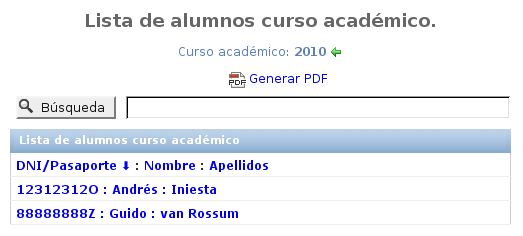
\includegraphics[scale=0.55]{4.Funcionamiento_Aplicacion/4.3.Gestion/4.3.2.Administrador_Centro/4.3.2.6.AlumnoCA/lista_alumnosCA.png}
      }
      \caption{Captura de pantalla de la lista de alumnos curso académico para el usuario \textit{Administrador de centro}.}
      \label{capturaPantallaListaAlumnosCAAdminCentro}
    \end{center}
  \end{figure}

  \paragraph{}Si se quisiera refinar el listado de elementos mostrados, es
  posible seleccionar nuevos parámetros pulsando el icono \textit{Seleccionar}
  que aparece al lado de cada elemento. Este icono aparece en la figura
  \ref{capturaBotonSeleccionar}.